\documentclass[10pt,a4paper]{article}
\usepackage[utf8]{inputenc}
\usepackage[french]{babel}
\usepackage[T1]{fontenc}
\usepackage{amsmath}
\usepackage{amsfonts}
\usepackage{amssymb}
\usepackage{graphicx}

\usepackage{algorithm}
\usepackage{algorithmic}

\usepackage{libertine}
\setlength{\parindent}{0cm}
\setlength{\parskip}{1ex plus 0.5ex minus 0.2ex}
\newcommand{\hsp}{\hspace{20pt}}
\newcommand{\HRule}{\rule{\linewidth}{0.5mm}}

\floatname{algorithm}{Algorithme}
\renewcommand{\algorithmicrequire}{\textbf{Entrée:}}
\renewcommand{\algorithmicensure}{\textbf{Sortie:}}
\renewcommand{\algorithmicif}{\textbf{si}}
\renewcommand{\algorithmicthen}{\textbf{alors}}
\renewcommand{\algorithmicelse}{\textbf{sinon}}

\begin{document}

\begin{titlepage}
  \begin{sffamily}
  \begin{center}

    % Upper part of the page. The '~' is needed because \\
    % only works if a paragraph has started.
    
\includegraphics[scale=0.15]{images/tree.jpg}~\\[1.5cm]

    \textsc{\LARGE U-MONS}\\[2cm]

    \textsc{\Large Rapport de projet de Structures de données 2}\\[1.5cm]

    % Title
    \HRule \\[0.4cm]
    { \huge \bfseries Priority Search Tree and Windowing\\[0.4cm] }

    \HRule \\[2cm]
    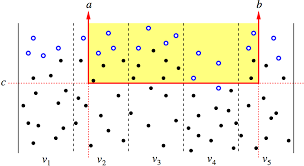
\includegraphics[scale=0.50]{images/window.png}
    \\[2cm]

    % Author and supervisor
    \begin{minipage}{0.4\textwidth}
      \begin{flushleft} \large
        \emph{\textbf{Directeurs :}}\\ G.Devillez et V.Bruyère\\
      \end{flushleft}
    \end{minipage}
    \begin{minipage}{0.4\textwidth}
      \begin{flushright} \large
        \emph{\textbf{Groupe :}}\\ M.Salemi et A.Lecocq
      \end{flushright}
    \end{minipage}

    \vfill

    % Bottom of the page
    {\large \today}

  \end{center}
  \end{sffamily}
\end{titlepage}

\newpage
\tableofcontents
\newpage
\section{Introduction}
Dans le cadre du cours de structures de données 2, nous avons été amenés à réaliser un projet en Java. Ce projet a pour objectif de créer et manipuler une structure de données non vue au cours. Cette nouvelle structure se base sur un arbre de recherche à priorité (Priority Search Tree en anglais ou PST). De la documentation nous a été fournie afin de nous familiariser avec cette dernière structure qui elle non plus n'a pas été vue au cours.

Un PST partage certaines caractéristiques avec les tas et les Arbres Binaires de Recherche ou ABR. Ces deux dernières structures de données ayant été étudiées en profondeur lors des séances de cours, nous les considérons ici comme connues.

\section{Présentation du problème}
Il nous a été demandé d'écrire un programme qui permette d'appliquer un "windowing" à un ensemble de segments de droite verticaux et horizontaux dans $\mathbb{R}^2$. Le windowing est une technique qui consiste à extraire tous les segments qui sont visibles dans une fenêtre donnée. Les différentes fenêtres à implémenter sont les suivantes :
\begin{itemize}
	\item $[X, X']$ x $[Y, Y']$ ;
	\item $[-\infty, X']$ x $[Y, Y']$ ;
	\item $[X, +\infty]$ x $[Y, Y']$ ;
	\item $[X, X']$ x $[-\infty, Y']$ ;
	\item $[X, X']$ x $[Y, +\infty]$.
\end{itemize}
La structure de données à implémenter devrait donc permettre un windowing efficace pour l'ensemble de ses fenêtres.


\newpage
\section{Priority Search Tree}

\subsection{Objectif de la structure}
Un PST est une structure de données de type arbre binaire (chaque nœud comporte au plus deux fils). Cette structure de données organise des points de l'espace défini par deux coordonnées X et Y. L'organisation des données permet d'effectuer efficacement la recherche des points présents dans une fenêtre de l'espace (sans avoir à parcourir l'ensemble des points).

\subsection{Définition}
Un PST est une structure de données mixte. Chaque nœud est constitué d'un point et d'un nombre appelé la médiane. Si l'on considère uniquement les coordonnées X, un PST est un tas avec le minimum à la racine. Si l'on considère uniquement les coordonnées Y, le PST est un ABR avec une petite particularité. Au lieu de trier les fils par rapport à la donnée du nœud courant, un PST trie les fils en fonction de la médiane du nœud courant.

Ainsi, tout nœud n d'un PST respecte les contraintes suivantes :
\begin{itemize}
	\item son fils gauche (s'il existe ainsi que ses descendants s'ils existent) aura sa coordonnée X plus grande que celle du nœud n et sa coordonnée Y plus petite que la médiane du nœud n ;
	\item son fils droit (s'il existe ainsi que ses descendants s'ils existent) aura sa coordonnée X plus grande que celle du nœud n et sa coordonnée Y plus grande que la médiane du nœud n.
\end{itemize}

\subsection{Construction}

\subsubsection{Tri des données}
La construction d'un PST est plus simple si l'on construit ce dernier à partir d'une liste de points triés selon la coordonnée Y. La première étape est donc de trier les points.

\subsubsection{Création de l'arbre}
Pour créer un arbre, créons le nœud racine à partir de la liste des points triés.

\subsubsection{Création d'un nœud}
La coordonnée X d'un nœud devant être plus petite ou égale à celle de ses fils, commençons par rechercher le point avec la plus petite coordonnée X. Attribuons ce point au nœud courant. Séparons le reste des points en deux. Attribuons comme médiane du nœud courant, la moyenne de la coordonnée Y du dernier point de la partie 1 et du premier point de la partie 2. Les points étant triés selon la coordonnée Y, la première partie est dispose d'une coordonnée Y plus petite ou égale à la médiane du nœud alors que la deuxième partie aura une coordonnée Y plus grande ou égale à la médiane du nœud. Dans le cas où il ne reste aucun point après le retrait du minimum en X, la valeur de la moyenne n'a pas d'importance. Dans le cas où il ne reste qu'un point, la coordonnée Y du point restant peut être attribuée à la médiane du nœud.

% TODO insert code

% TODO better explain windowing
\subsection{Windowing}
Le windowing est une technique très répandue qui consiste à sélectionner une certaine fenêtre parmis une énorme quantité de données. Un exemple pratique très répandu est l'affichage d'une carte sur un gps, le gps se voulant rapide n'affichera pas toutes les routes qui se trouvent dans le monde(énorme quantité de données) mais seulement celles qui nous entourent au moment où  nous roulons avec notre véhicule.


\newpage
\section{PST Adapté}
Étant donné que notre windowing s'applique à des segments et non à des points, nous ne pouvons utiliser le PST tel que décrit ci-dessus. Nous avons donc adapté cette structure afin de permettre l'utilisation de segments.

Un segment est défini par 2 points, chacun ayant une coordonnée X et une coordonnée Y. Un segment possède donc 2 coordonnées X ainsi que 2 coordonnées Y. Un segment est soit horizontal soit vertical, c'est-à-dire soit les coordonnées X soit les coordonnées Y sont égales.

Afin de garder les explications concises et faciles à comprendre, nous allons d'abord considérer uniquement une fenêtre de type $[X, X']$ x $[Y, Y']$ ou $[-\infty, X']$ x $[Y, Y']$ et nous expliquerons ensuite comment gérer les autres cas.

\subsection{Objectif de la structure}
L'objectif de cette structure est d'organiser l'ensemble des segments afin de faciliter la recherche de segments visibles dans une fenêtre de type $[X, X']$ x $[Y, Y']$ ou $[-\infty, X']$ x $[Y, Y']$.

\subsection{Définition}
Notre PST adapté respecte exactement la définition d'un PST excepté 2 adaptation :
\begin{itemize}
	\item un segment sera stoqué par nœud au lieu d'un point ;
	\item les coordonnées utilisées pour effectuer la comparaison sont le minimum des coordonnées X du segment comme X, le minimum des coordonnées Y du segment comme Y.
\end{itemize}

Le choix des coordonnées de référence est judicieux car il permet lors de la recherche d'une fenêtre, d'élaguer tout nœud (ainsi que ses descendants par définition du tas) dont la coordonnée minimum en X est supérieure à X' et il permet de ne pas visiter le fils droit (ainsi que ses descendants par définition de l'ABR) de tout nœud dont la médiane est strictement supérieure à Y'.

\subsection{Construction}
Notre PST adapté se construit à la manière d'un PST excepté que les références pour la comparaison des données sont les coordonnées minimums en X ainsi qu'en Y. C'est-à-dire que nous trions les segments selon leur plus petite coordonnée en Y. Lorsque nous recherchons le minimum en X, nous recherchons le segment avec la plus petite coordonnée X.

\subsection{Windowing}
Étant donné que nous devons reporter tous les segments visible dans une certaine fenêtre, nous devons non seulement extraire les segments ayant un point dans la fenêtre, mais aussi les segments commençant avant et finissant après. C'est le cas notamment du segment possédant les coordonnées (X'-1, Y-1) (X'-1, Y'+1). La recherche sera donc un peut moins efficace que pour les points et nous allons devoir utiliser une approche différente.

Nouvelle approche : se concentrer sur le point de départ du segment c'est-à-dire le point ayant la plus petite coordonnée X pour un segment horizontal, le point ayant la plus petite coordonnée Y pour un segment vertical. Nous avons ici 3 possibilités pour que le segment soit visible :
\begin{itemize}
	\item soit le point de départ est dans la fenêtre ;
	\item soit le point de départ est à gauche de la fenêtre et le segment traverse la limite gauche de la fenêtre ;
	\item soit le point de départ est en dessous de la fenêtre et le segment traverse la limite basse de la fenêtre.
\end{itemize}
Il est évident que si le point de départ se situe au dessus ou à droite de la fenêtre, ce segment ne sera pas visible dans la fenêtre.
% TODO add schema of the window to help comprehension

Nous allons donc parcourir l'arbre à partir de la racine et le traiter de la sorte :
\begin{itemize}
	\item si le minimum en X du segment est strictement supérieur à X', alors on laisse tomber ce nœud ainsi que tous ses descendants (le segment de ce nœud ainsi que celui de ses descendants a son point de départ à droite de la fenêtre) ;
	% TODO add reference to ci-desssus
	\item si ce segment est visible dans la fenêtre (voir conditions ci-dessus), le reporter ;
	\item si la médiane du nœud est strictement supérieure à Y' (le segment du fils droit ainsi que celui de ses descendants a son point de départ au dessus de la fenêtre), alors parcourir le fils gauche uniquement sinon parcourir les deux fils.
\end{itemize}
% TODO image de l'arbre et des noeud parcourus

% TODO insert code ?
L'utilisation de cette structure pour réaliser un windowing de type $[-\infty, X']$ x $[Y, Y']$ est très efficace car aucun nœud inutile n'est parcouru.


\subsection{Les autres fenêtres}
\subsubsection{De $[-\infty, X']$ x $[Y, Y']$ à $[X, X']$ x $[-\infty, Y']$}
Nous avons vu une structure de données très efficace pour réaliser un windowing de type $[-\infty, X']$ x $[Y, Y']$. Cependant, nous devons également réaliser un windowing avec une fenêtre de type $[X, X']$ x $[-\infty, Y']$. Nous remarquons que pour obtenir cette fenêtre efficacement, il suffit d'échanger les coordonnées X et Y. Nous aurions pu implémenter une structure de donnée supplémentaire étant un tas selon Y et un ABR selon X (avec les médianes). Nous avons choisi de réutiliser la même structure de données et d'inverser les coordonnées des segments avant la construction de l'arbre. Ainsi le segment (X, X'),(Y, Y') devient après échange le segment (Y, Y'),(X, X'). Nous effectuons une recherche avec la fenêtre échangée $[-\infty, Y']$ x $[X, X']$ et effectuons un échange inverse sur les segments reportés afin de retrouver les segments originaux.

\subsubsection{Les autres fenêtres semi-infinies}
Maintenant que nous pouvons effectuer une recherche efficace sur des fenêtres de type $[-\infty, X']$ x $[Y, Y']$ et $[X, X']$ x $[-\infty, Y']$, il nous reste les fenêtres $[X, +\infty]$ x $[Y, Y']$et $[X, X']$ x $[Y, +\infty]$. Nous remarquons que pour obtenir ces fenêtres efficacement, il suffit d'opposer les coordonnées. Nous aurions pu ici aussi créer une structure de donnée avec une comparaison différente. Nous avons également choisi de réutiliser la même structure et d'opposer les coordonnées avant la construction de l'arbre. Ainsi, le segment (X, X'),(Y,Y') devient après opposition (-X',-X),(-Y',-Y).

\subsubsection{La fenêtre fermée}
Lors de la recherche dans une fenêtre fermée avec l'arbre décrit ci-dessus, nous ne pouvons jamais éliminer le fils gauche de nos recherches. En conséquence, les nœuds que nous parcourons ayant un minimum en X strictement inférieur au X de la fenêtre et ayant un minimum en Y strictement inférieur au Y de la fenêtre sont parcourus inutilement. Ces segment sont ceux qui commencent en bas à gauche de la fenêtre et il est évident qu'ils n'y seront pas visibles. Nous avons donc adapté notre windowing afin qu'il prenne deux paramètre :
\begin{itemize}
	\item center : définit si les segments commençant au centre de la fenêtre doivent être reportés ;
	\item down : définit si les segments commençant en dessous de la fenêtre doivent être reportés.
\end{itemize}
Si center est faux, alors nous pouvons laisser tomber les nœuds qui ont un minimum en X plus grand que le X de la fenêtre.
Si down est faux, alors nous pouvons laisser tomber les fils gauches des nœuds dont la médiane est strictement inférieure au Y de la fenêtre.

Afin d'effectuer la recherche de la fenêtre fermée efficacement, nous appliquerons le windowing deux fois. Une première fois avec down à faux afin de reporter les segments ayant le point de départ à gauche et dans la fenêtre. Une seconde fois sur la fenêtre échangée avec la même technique que pour la fenêtre $[X, X']$ x $[-\infty, Y']$ avec center et down à faux afin de reporter tous les segments ayant leur point de départ en dessous.

\section{Diagrammes de classes}
\subsection{Pst et BasicPst}
BasicPst correspond au PST gérant efficacement une fenêtre de type $[-\infty, X']$ x $[Y, Y']$. Afin de gérer toutes les transformations, nous avons créé une autre classe Pst qui comporte 4 BasicPst :
	\item un avec les segments originaux pour les fenêtres $[-\infty, X']$ x $[Y, Y']$ ;
	\item un avec les segments échangés pour les fenêtres $[X, X']$ x $[-\infty, Y']$ ;
	\item un avec les segments opposés pour les fenêtres $[X, +\infty]$ x $[Y, Y']$ ;
	\item un avec les segments échangés et opposés pour les fenêtres $[X, X']$ x $[Y, +\infty]$ ;
\end{enumerate}

Cette classe s'occupe de choisir l'arbre sur lequel effectuer le windowing afin d'obtenir la meilleure efficacité.

\subsection{Diagramme de classe des données}
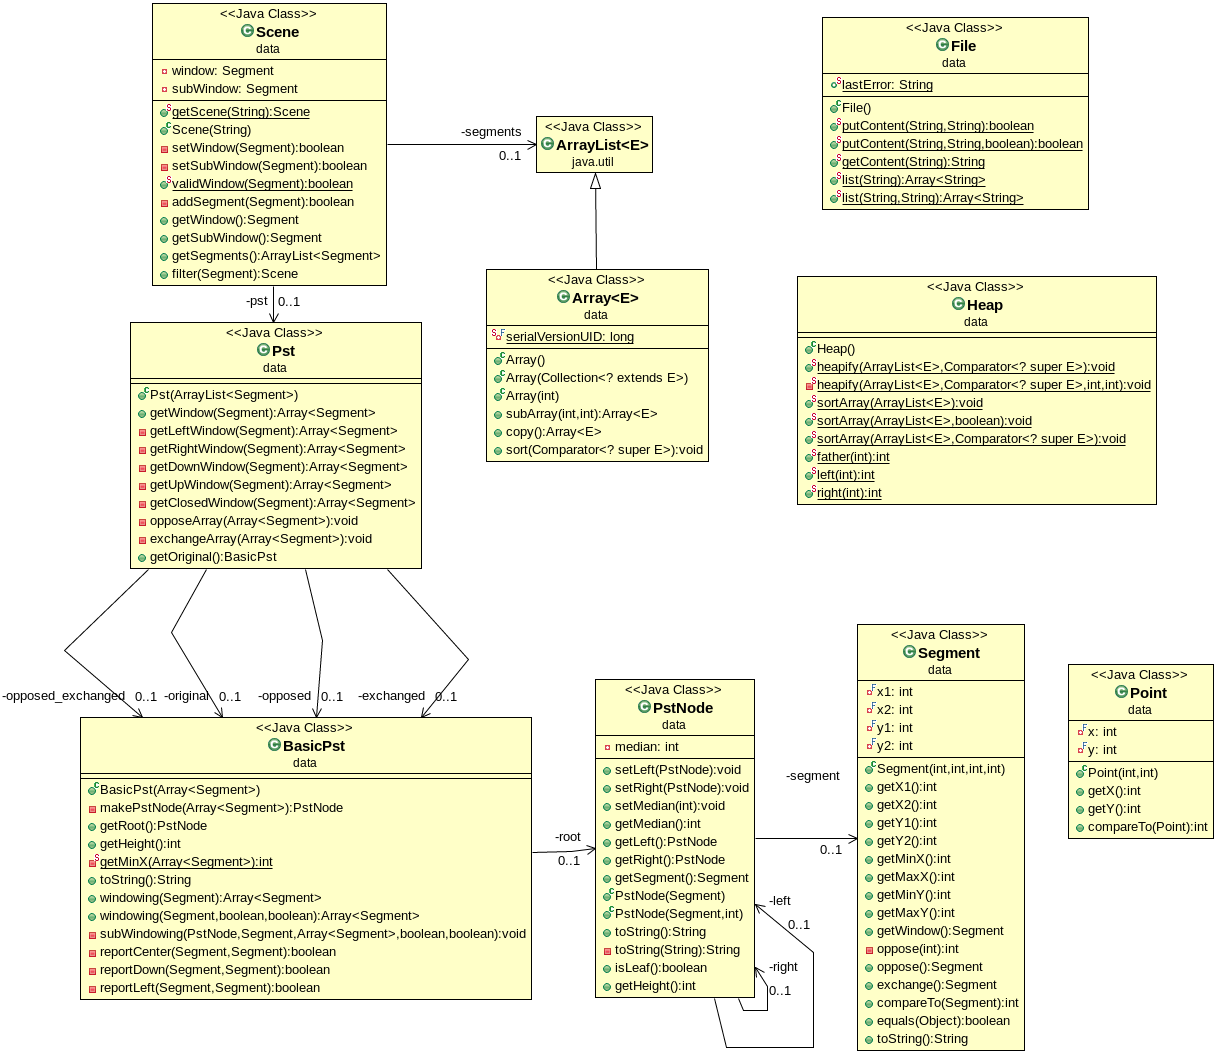
\includegraphics[scale=0.3]{../src/UML/data.png}

\subsection{Diagramme de classe de l'interface graphique}
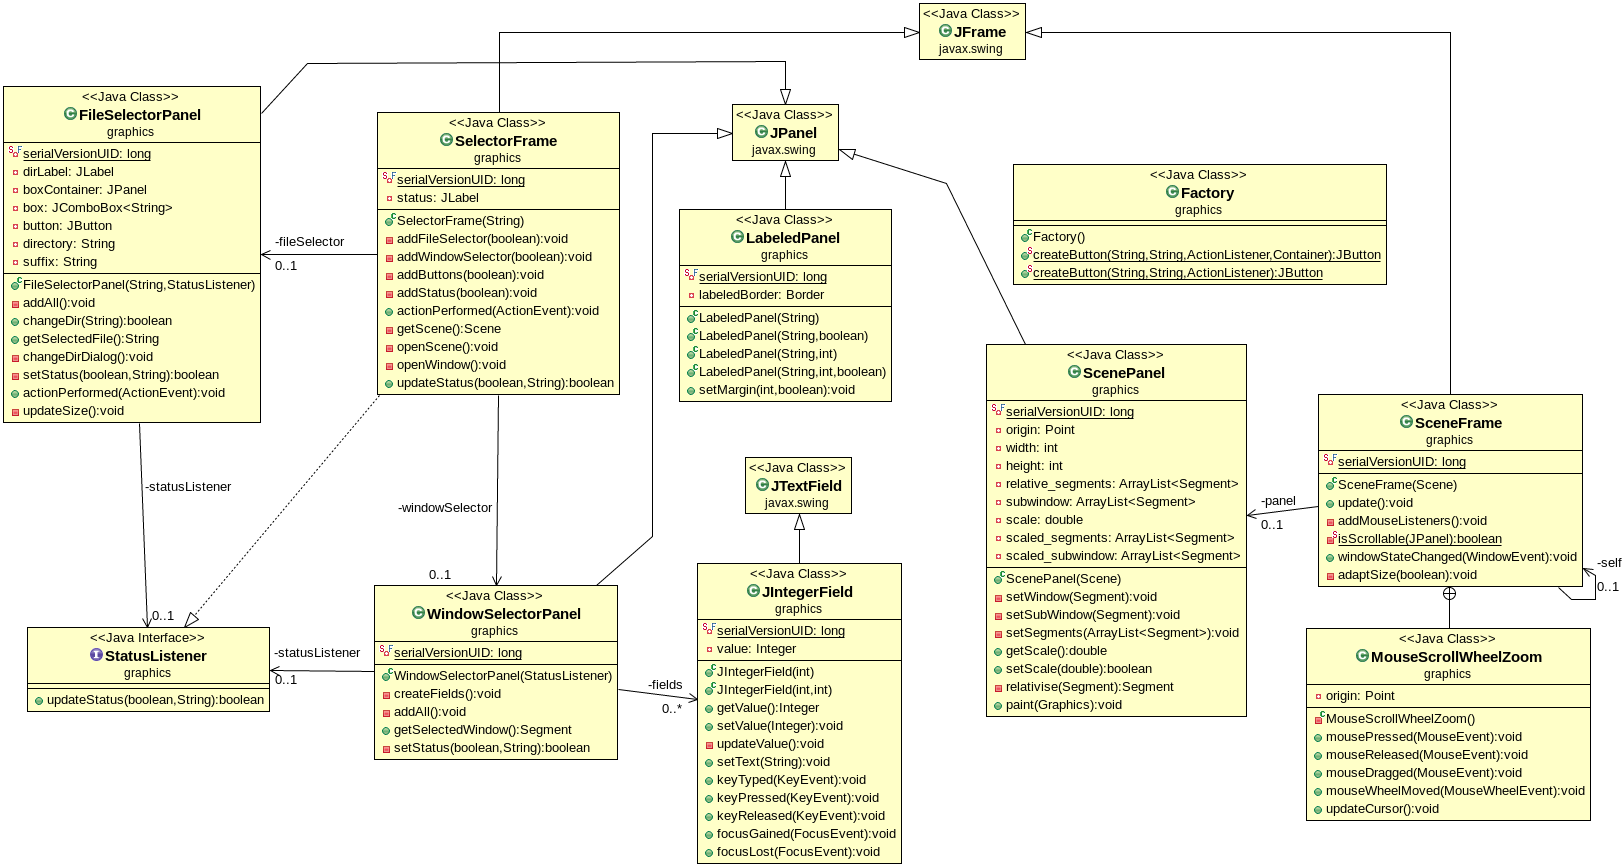
\includegraphics[scale=0.25]{../src/UML/graphics.png}

\section{Idées et Mise en pratique}
\subsection{Passage des points au segments}

\section{Diagramme de Classes}

\section{Algorithmes et explications}
Dans cette section, nous exposons nos différents algorithmes importants en pseudo-code ainsi que leur complexité en temps. Une courte explication en français y est aussi ajoutée afin de favoriser la compréhension de ceux-ci et leurs utilisations.
\subsection{Construction de l'arbre}

\begin{algorithm}
\caption{Construction de l'arbre}
\begin{algorithmic}[1]
\REQUIRE une liste de Segment $A$
\ENSURE /
\STATE $max \leftarrow -\infty$
\FOR{$i \leftarrow 1$ à $longueur[A]$}
\IF{$max < A[i]$}
\STATE $max \leftarrow A[i]$
\ENDIF
\ENDFOR
\RETURN $max$
\end{algorithmic}
\end{algorithm}


\section{Démonstrations}
Durant cette section, nous allons démontrer certaines propriétés du Pst qui ne sont pas couvertes par nos algorithmes(certaines preuves ont été réalisées lors des tests).
\subsection{Arbre équilibré}

\subsection{Transformation des fenêtres}

\section{Illustrations}
Ce point du rapport sert d'illustration, vous permettant d'observer différents cas d'exemples d'application du windowing, et ceci via l'application que nous avons créer.

\section{Mode d'emploi}
Après vous avoir montrer en images notre application, nous vous expliquant ici comment faire fonctionner notre application. Vous pourrez ainsi constater cette réelle application par vous-même, qui est très intuitive et parfaitement fonctionnelle.

\section{Conclusion}


\end{document}